% GravExplain
\documentclass[prb,preprint]{revtex4-1} 
% \documentclass[prb,preprint,letterpaper,noeprint,longbibliography,nodoi,footinbib]{revtex4-1} 

% Note that AJP uses the same style as Phys. Rev. B (prb).
% The AIP Style Manual\cite{AIPstylemanual} is an indispensable reference on good physics writing, covering everything from planning and organization to standard spellings and abbreviations.
% Most important of all, please familiarize yourself with the AJP Statement of Editorial Policy,\cite{editorsite} which describes the types of manuscripts that AJP publishes and the audience for which AJP authors are expected to write.
% We look forward to receiving your submission to AJP.
\usepackage[utf8]{inputenc}
\usepackage{amsmath,amssymb,amsthm}
\usepackage{amsfonts}
\usepackage{graphicx}
\usepackage{float}
\usepackage{mathtools}
\usepackage[usenames,dvipsnames]{xcolor}
\usepackage{hyperref}
% \usepackage{siunitx}

\bibliographystyle{apsrev4-2}
% \setlength{\parindent}{0pt}

\newcommand{\jam}{\textcolor{magenta}}
\newcommand{\han}{\textcolor{orange}}


\begin{document}

% cover page
\section*{Project contributions}
% contributions clarify what’s to be assessed
James W. Gardner:
\begin{itemize}
\item all paper sections other than the introduction, i.e.\ from Section~\ref{sec:ifo} onwards, and all figures in the paper
\item addition of the injection speaker, design of photodiode circuit from standard examples, assembly of circuit on breadboard, and set-up of Raspberry Pi to measure output
\item all of the source code at \url{https://github.com/daccordeon/gravexplain}, that reads the data from the Raspberry Pi, analyses it, and creates the figures used in the paper
\item talks presented were based on paper and figures therein
\end{itemize}

Hannah Middleton:
\begin{itemize}
\item introduction of paper, i.e.\ Section~\ref{sec:introduction}
\item design and assembly of the interferometer
\end{itemize}

Andrew Melatos, Robin Evans, William Moran: vital advice and comments throughout the project

\subsection*{Statement of achievements}
% one paragraph recount of what’s been done for two months, like the abstract

\jam{write this!}

\newpage

\title{GravExplain: Continuous gravitational wave searches in a table-top experiment}

\author{James W. Gardner}
\email{u6069809@anu.edu.au}
\affiliation{Research School of Physics, Australian National University, 60 Mills Rd, Acton ACT 2601 Australia}

\author{Hannah Middleton$^{(i)}$}
\email{hannah.middleton@unimelb.edu.au}
\author{Andrew Melatos$^{(i)}$}
\email{amelatos@unimelb.edu.au}
\author{Robin Evans$^{(ii)}$}
\email{robinje@unimelb.edu.au}
\author{William Moran$^{(ii)}$}
\email{wmoran@unimelb.edu.au}
\affiliation{School of Physics$^{(i)}$ and Department of Electrical and Electronic Engineering$^{(ii)}$, University of Melbourne, Parkville, VIC, 3010, Australia}
\affiliation{OzGrav-Melbourne, Australian Research Council Centre of Excellence for Gravitational Wave Discovery}

% Summer 2019/2020
\date{\today}

% AJP requires an abstract for all regular article submissions.
\begin{abstract}
Continuous gravitational wave searches use sophisticated statistical techniques to search for signals in noisy data. We demonstrate some of these techniques with a table-top Michelson interferometer, namely the Viterbi algorithm for recovering a tone with wandering frequency.
We also use the same experiment to demonstrate an optical microphone capable of playing back simple audio recordings of injected music. However, played-back speech is currently unintelligible so we investigate preliminary methods of speech enhancement.
 
\jam{Andrew says that this should be a bit more detailed!}

\end{abstract}

\maketitle

\section{Introduction}
\label{sec:introduction}

% general gw intro
In 2015 gravitational waves were observed for the first time from the merger of two black holes in a binary system.~\cite{GW150914} 
The observation, made by the Laser Interferometer Gravitational-wave Observatory~\citep[LIGO]{AdvancedLIGO:2015}, marked a breakthrough in modern astrophysics and provides a new means to observe the universe. 
Since 2015, the LIGO and Virgo~\cite{AdvancedVirgo:2015} observatories have made numerous detections of binary black hole~\cite{GW151226,GW170104,GW170814} and binary neutron star~\cite{GW170817,GW170817multi,GW190425} mergers. 
In recent years there has been an increased public interest in gravitational-wave science. 
Many gravitational wave research groups around the world have produced demonstrations and activities to aid in explaining this topic to a general audience.
Activities range from online data analysis tutorials,~\cite{GWOSC:online,LOSC:2015} hands-on demonstrations, phone apps,~\cite{LaserLabs:online,SciVR:online} and online games,~\cite{BlackHoleHunter:online} to exhibitions,\cite{L2URSSE} artistic interpretation, and musical performance~\cite{ArthurJeffesMusic:online,GravitySynthLeonTrimble:online}. 

% what are gws and how do we detect them...
Gravitational waves are a prediction of Einstein's theory of general relativity. 
They are disturbances in spacetime caused by the acceleration of massive objects. 
The effect of gravitational waves is a change in distances; a ``stretch and squeeze'' effect. 
Observatories such as LIGO, Virgo, and KAGRA~\cite{KAGRA:2013} are laser interferometers; they use the interference of laser light to measure changes in distance. 
Gravitational-wave observatories are extremely complex devices, however they are based on the Michelson interferometer. 
Table-top Michelson interferometers are commonly used by gravitational-wave research groups to demonstrate the science of gravitational-wave detection to non-specialist audiences~\cite{ThorLabsIFO,NikhefIFO,ExhibitIFO,LIGOIFOGlue,LIGOIFOMagnets} and they are often used in undergraduate lab experiments~\cite{UgoliniEtAl:2019}. 

% continuous gws
To date the network of gravitational-wave observatories have observed short-duration transient signals~\cite{GWTC-1:2018,GWOSC:online}. 
These observatories are also searching for continuous gravitational waves (CW); persistent periodic signals at near-monochromatic frequencis. 
One of the prime targets of CW searches are rotating neutron stars in low mass X-ray binaries (LMXBs).
LMXBs are binary systms containing a compact object (such as a neturon star or a black hole) in orbit with a low mass stellar companion~\cite{xraybinaries:1997}. 
The LMXB Scorpius X-1 is an LMXB which is particularly bright in X-rays. 
It is a prime target for CW searches from LMXBs and numerous searches have been performed~\cite{2019PhRvD.100l2002A,RadiometerO1O2:2019,SearchCrossCorrO1:2017}. 
 
% sound analogy
Here we demonstrate the use of a Michelson interferometer as a tool to explain the search for continuous waves to a general audience.
The analogy of listening to the universe is often used to explain gravitational-wave observations; transient gravitational-wave signals have been converted into audio.
Continuous waves may emitt at constant frequencies, or they may wander slowly in frequency over time. 
This can be demonstrated with a table-top interferometer by playing audio of constant or slowly changing frequency tones to produce a simulation of a continuous wave signal. 
The analysis techniques used in this work are similar to those used to search for continuous gravitational waves in LIGO and Virgo data, particularly for the wandering frequency demonstration~\cite{ScoX1ViterbiO2,ScoX1ViterbiO1:2017,SuvorovaEtAl:2017,SuvorovaEtAl:2017}. 

In this work we detail our table-top intererometer design in Section~\ref{sec:ifo}, in Section~\ref{sec:single_tone} we describe observing a single tone signal, Section~\ref{sec:viterbi_wandering} describes observing a wandering frequency signal, and Section~\ref{sec:optical_microphone} extends the set-up to be able to capture complex audio, such as music and speech. We suggest avenues of future work in Section~\ref{sec:future_work} and draw conclusions in Section~\ref{sec:conclusions}.


% \section{Method and results}
\section{Table-top gravitational wave science}
\label{sec:ifo}

Detectable gravitational waves are caused by some of the most violent events in the universe. Like two massive black-holes merging with each other\cite{GW150914}. Even so, the effects they produce are on the order of one part in $10^{21}$ for our best detectors\cite{GW150914}. For a table-top experiment these effects would be far too small, so we demonstrate observing a far louder source, sound waves. Although the analogue to gravitational waves is tenuous, we can still demonstrate some of the continuous wave analysis satisfactorily. The other benefit of observing sound is that we can use existing signal processing techniques designed for audio signals.

\subsection{Michelson interferometry}
% hardware: path difference, virtual thin film interference

A Michelson interferometer is a well-known optics configuration used in many undergraduate and research labs, including in the detectors for gravitational waves. A laser beam of coherent (monochromatic and equal phase) light is split evenly by a 50/50 beamsplitter into two arms at right-angles to each other, travelling down and back from a mirror at the end of each arm. The beams recombine and interfere at the beamsplitter before hitting a screen to produce a pattern of concentric, circular fringes. The configuration is shown in Figure~\ref{fig:ifo_schematic_webcam}. In the detectors for gravitational waves, these arms are kilometres long and many other complexities (such as power recycling and quantum squeezing)\cite{GW150914} are necessary to observe a signal.

\begin{figure}
	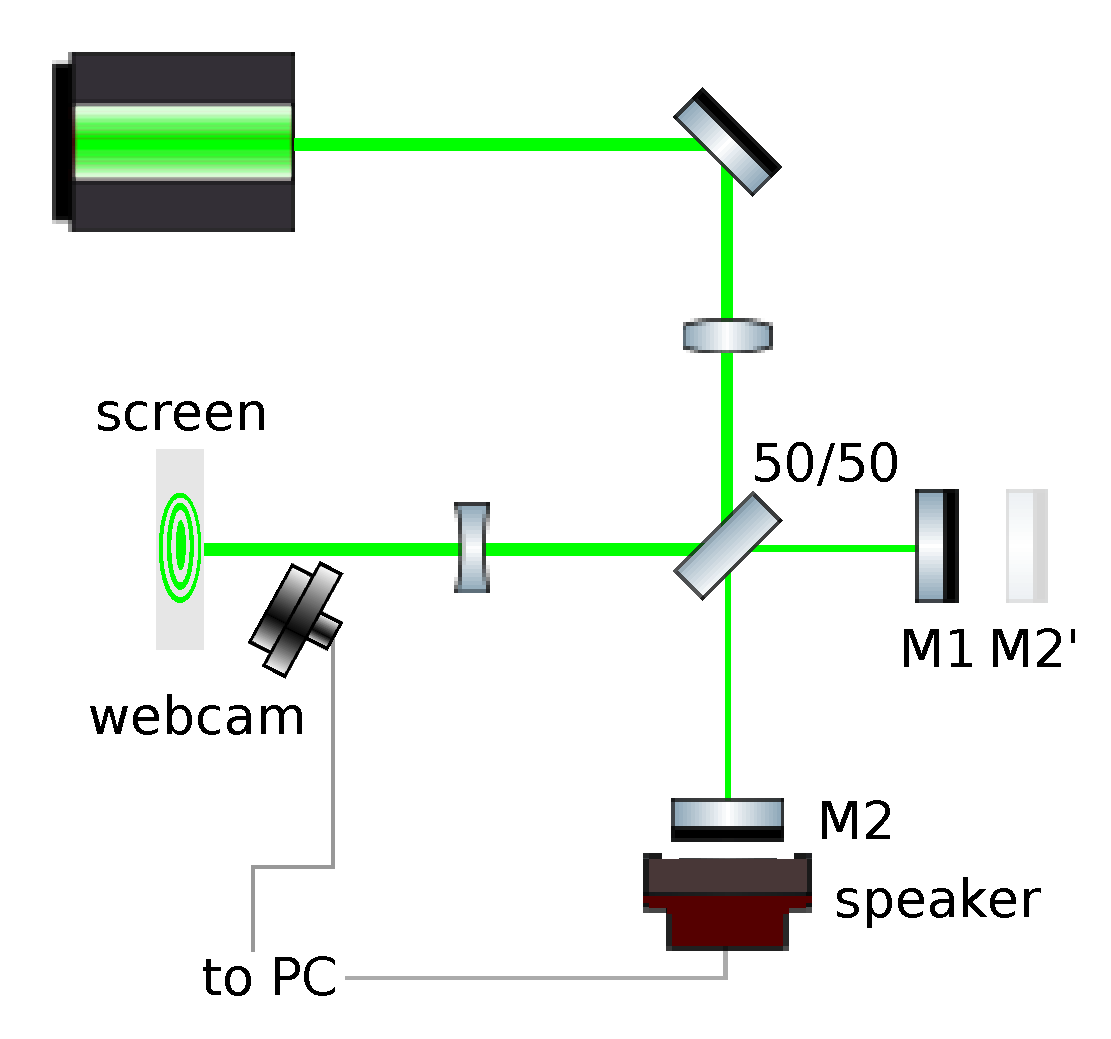
\includegraphics[width=0.8\textwidth]{figures/ifo_schematic_webcam.pdf}
	\caption{Michelson interferometer schematic, interference pattern is recorded by a webcam}
	\label{fig:ifo_schematic_webcam}
\end{figure}
% Note that we do not include the common compensating plate that equalises the amount of time spent in glass for each beam. We did not find it necessary to include it to be able to demonstrate the results desired.

The interference pattern, as shown in Figure~\ref{fig:interference_pattern}, is due to the path difference between the two arms of unequal lengths (if the lengths were equal, then only a single, bright dot would be seen). This results in a phase difference between the two beams when they meet at the screen. This path difference is perhaps better seen as the perpendicular separation between one mirror and the virtual image of the other.
For an aligned configuration and a fixed separation, the phase difference at a point only depends on the angle from the centre-line of the beam, and so the pattern is circularly symmetric.

\begin{figure}
	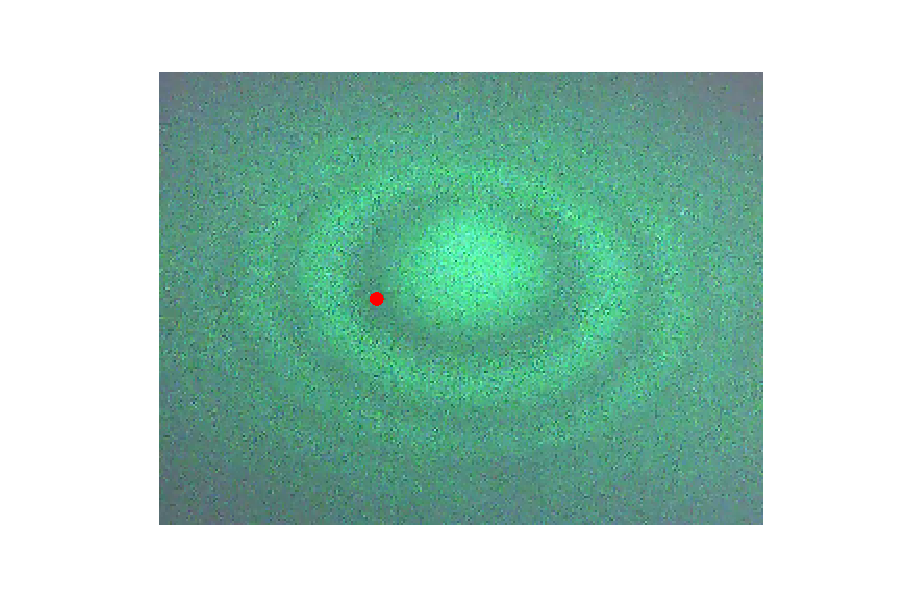
\includegraphics[width=\textwidth]{figures/webcam_still0.pdf}
	\caption{Interference pattern from Michelson interferometer as viewed by webcam from off-centre (hence why the pattern appears non-circular), red dot indicates point where intensity time series was measured from. For scale, the central fringe is approximately 5mm across}
	\label{fig:interference_pattern}
\end{figure}

% A note that while the interference pattern appears similar to the Airy pattern produced by a circular aperture, they are not in fact the same geometry.

\section{Observing a single tone}
\label{sec:single_tone}
% the webcam method
% how to analyse video, python OpenCV2

Continuous gravitational wave searches are, by the nature of the astrophysical sources that they look for, always searching for periodic, or even sinusoidal, signals. Often the frequency of this periodicity can change, as addressed later, but sometimes it is (near) constant. As such, the audio analogue is to observe a single tone (a sinusoidal note of one frequency).

\subsection{Method}

We use a 0.5W speaker stuck to the back of one of the mirrors as a source for our demonstration, as shown in Figure~\ref{fig:ifo_schematic_webcam}. This speaker was part of a commercial 3.5mm-jack, USB powered pair of speakers and is driven by a PC. Previously, we used a function generator to accomplish the same signal.
As the speaker deforms to play sound, the mirror moves with a change in separation, $\delta d$, as some coupling function of the amplitude and frequency of the sound. The motion of the fringes follows the motion of the mirror and therefore the speaker at the same frequency.
If the fringe motion is small, then changes in the intensity at some point on the screen follow the frequency of the injected (played) audio but with amplitude given by a transfer function that accounts for the coupling and resonance of the speaker-mirror system.
Large fringe motion means that multiple fringes can pass over the measured point in a single speaker deformation, such over-counting would artificially raise the measured frequency. As such, any motion of the fringes, and so of the speaker, must be kept small by playing sound softly through the speaker.


\subsection{Results}

We measure the intensity at a point on the screen with a commercial USB webcam placed as to view the screen (Figure~\ref{fig:ifo_schematic_webcam}), sampling at 30Hz (or 30 fps, frames-per-second). This limits the spectral content of signals we can observe to be under the Nyquist frequency of 15Hz.
See later Section~\ref{sec:photodiode} where we raise this limit into to audible frequencies (20 Hz to 20kHz) with a photodiode.
While playing a tone under 15Hz through the speaker for a minute, we recorded the interference pattern with the webcam. Then, at an off-centre pixel as seen in Figure~\ref{fig:interference_pattern}, we take the green-channel of the colour (RGB) video as approximate to the total intensity, as the laser is monochromatic green light. We can play this time series of intensity over time as an audio recording (we used the \textbf{scipy.io.wavfile.write}\cite{scipy} function in Python\cite{python}) and the tone is clearly heard.
Taking the Fourier transform of this signal shows the injected tone, as seen in Figure~\ref{fig:webcam_spectrum} where we record the highest peak Fourier amplitude at $(2.099\pm 0.008)\mathrm{Hz}$ for an injected tone of 2.09Hz (a result within two standard deviations).
Therefore, we’re able to observe a single tone quite confidently.

\begin{figure}
	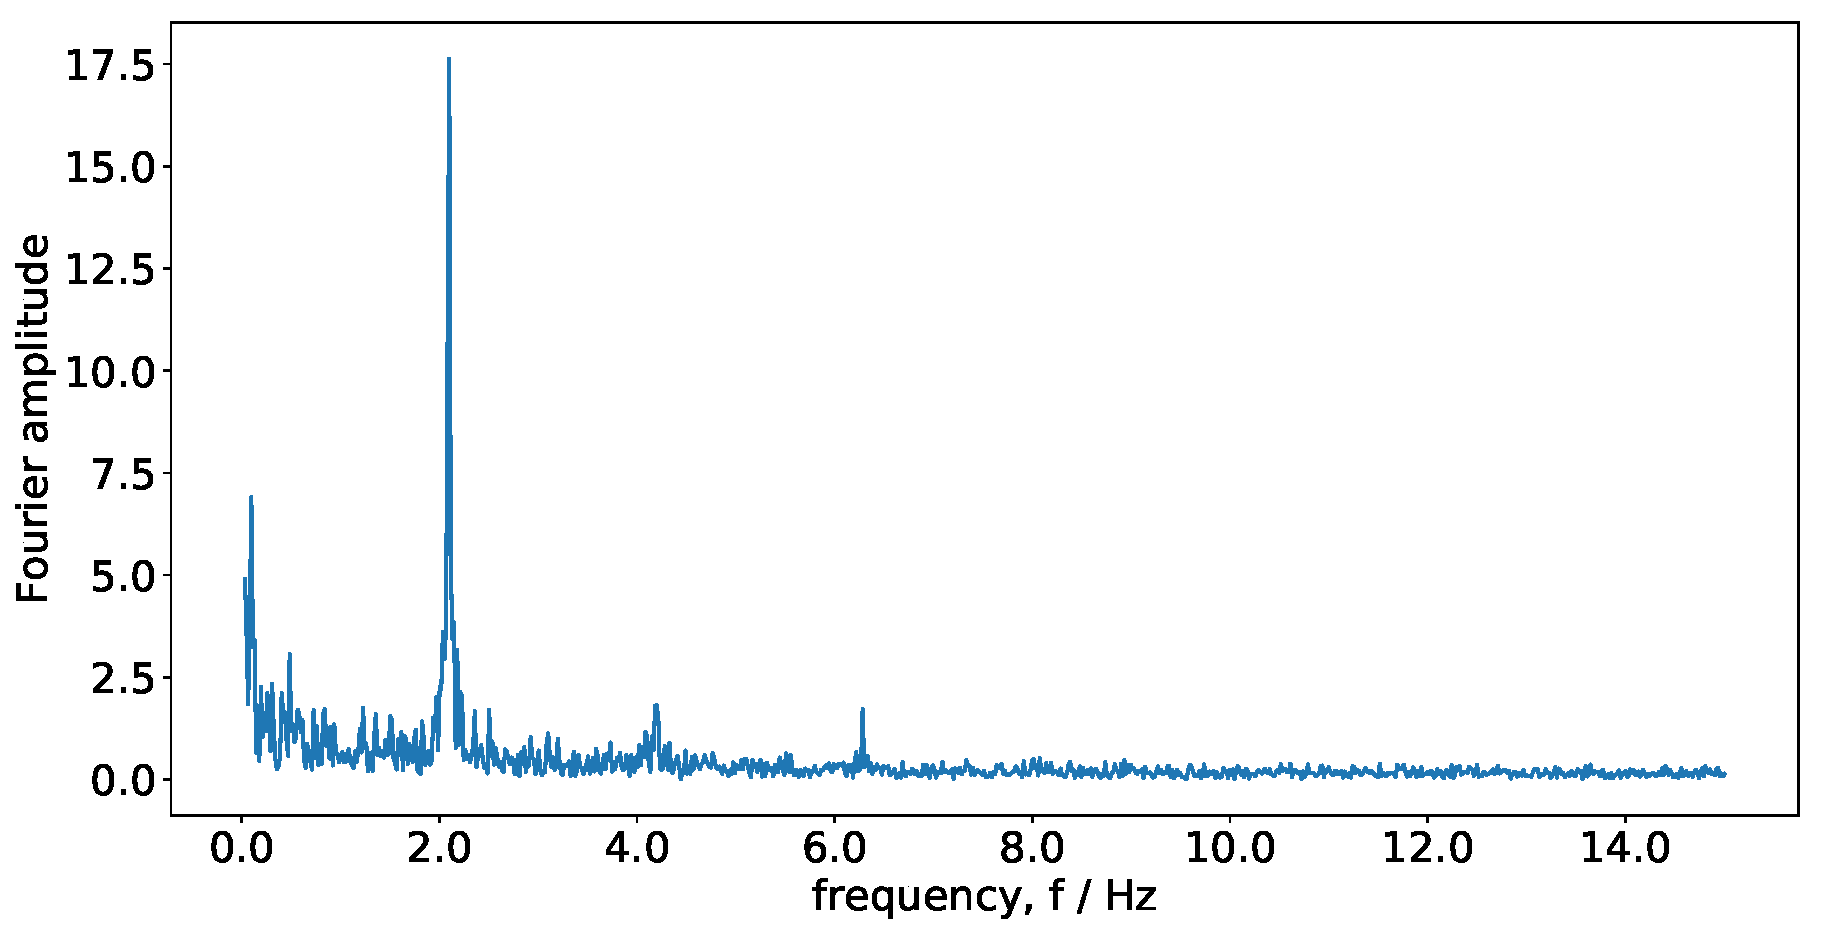
\includegraphics[width=\textwidth]{figures/webcam_expt_4_0209-cropped.pdf}
	\caption{Fourier amplitudes of intensity time series of interference pattern as captured by a webcam for an injected tone of 2.09Hz, the highest peak is measured at $(2.099\pm 0.008) \mathrm{Hz}$ for an injected tone of 2.09Hz. In fact, the actual highest peak is at 0Hz, but that corresponds only to a non-zero average value, so we don’t display or consider it.}
	\label{fig:webcam_spectrum}
\end{figure}

\section{Observing a wandering tone}
\label{sec:viterbi_wandering}
% Tracking tones with the Viterbi algorithm
% explaination and successful application
% lean on the continuous gravitational waves angle

Continuous gravitational wave searches often look for signals that wander (change) in frequency slowly over time\cite{2019PhRvD.100l2002A}. This means that finding the signal isn’t as simple as searching for a peak in the frequency content for the full observing run, especially when the signal-to-noise ratio is particularly low.

One method (among many) is to split the observed time series into bins of time, compute the Fourier transform for each time interval, and then create a grid (known as a spectrogram) where each cell is the Fourier amplitude of a particular frequency at a particular time.
The method then treats the problem as one of finding the best path through a weighted graph, where here the weights are given by the Fourier amplitudes.
The method takes in a parameter of the allowed frequency wandering, some rate of frequency change over time, usually informed by a physical model. Here, this parameter is set to 0.11 Hz per second to make it simply one frequency bin per every time bin, which will prove poorly adjusted to the signal.


\subsection{The Viterbi algorithm}

The Viterbi algorithm is a path-finding algorithm that solves this problem.
Abstractly speaking, the algorithm is given a weighted graph (e.g.\ the spectrogram grid), a sensible sequence of subgraphs (e.g.\ the columns holding spectrum at each time), and restrictions on connectivity (e.g.\ the allowed amount frequency wander). Then, at each iteration, it will find the best path to each node in the next subgraph, all the way from the first subgraph. At the end, it selects the overall best path from the first to the last subgraph (here, from the start to end time), this overall best path is called the Viterbi path. See Appendix~\ref{app:viterbi} for the full details of the algorithm in this particular implementation.

\subsection{Results}

We demonstrate this method of using the Viterbi algorithm to find a signal, by injecting a wandering frequency signal into the speaker and recording the output via the webcam.
Note that when creating a wandering frequency signal, the phase change must be integrated up over time, as detailed in Appendix~\ref{app:phase_gotcha}.

Shown in Figure~\ref{fig:viterbi_overlay} is the resultant spectrogram of the observed signal, overlaid with the injected signal and the recovered Viterbi path.
To the eye, the Viterbi algorithm easily recovers the injected frequency over time due to the high signal-to-noise ratio (SNR) of this experiment. Quantifying this, the Viterbi path stays within one frequency bin (approximately 0.3Hz) of the injected tone for 94\% of the run.
Note that the signal initially moves faster than the chosen frequency wander parameter, causing a discrepancy between the injected and recovered signals. To fix this, the parameter should be doubled, although this would then cause the recovered path to stray more often. There also appears to be an anomaly at 150s, likely from a disturbance (such as someone walking) around the interferometer.

Empirically, decreasing the signal-to-noise ratio closer to unity also causes the Viterbi algorithm to more easily stray from the signal to reach nearby fluctuations. However, the only correlation through the grid is the signal, so we always expect the Viterbi path to lie near to the signal no matter how high the noise is.

\begin{figure}
	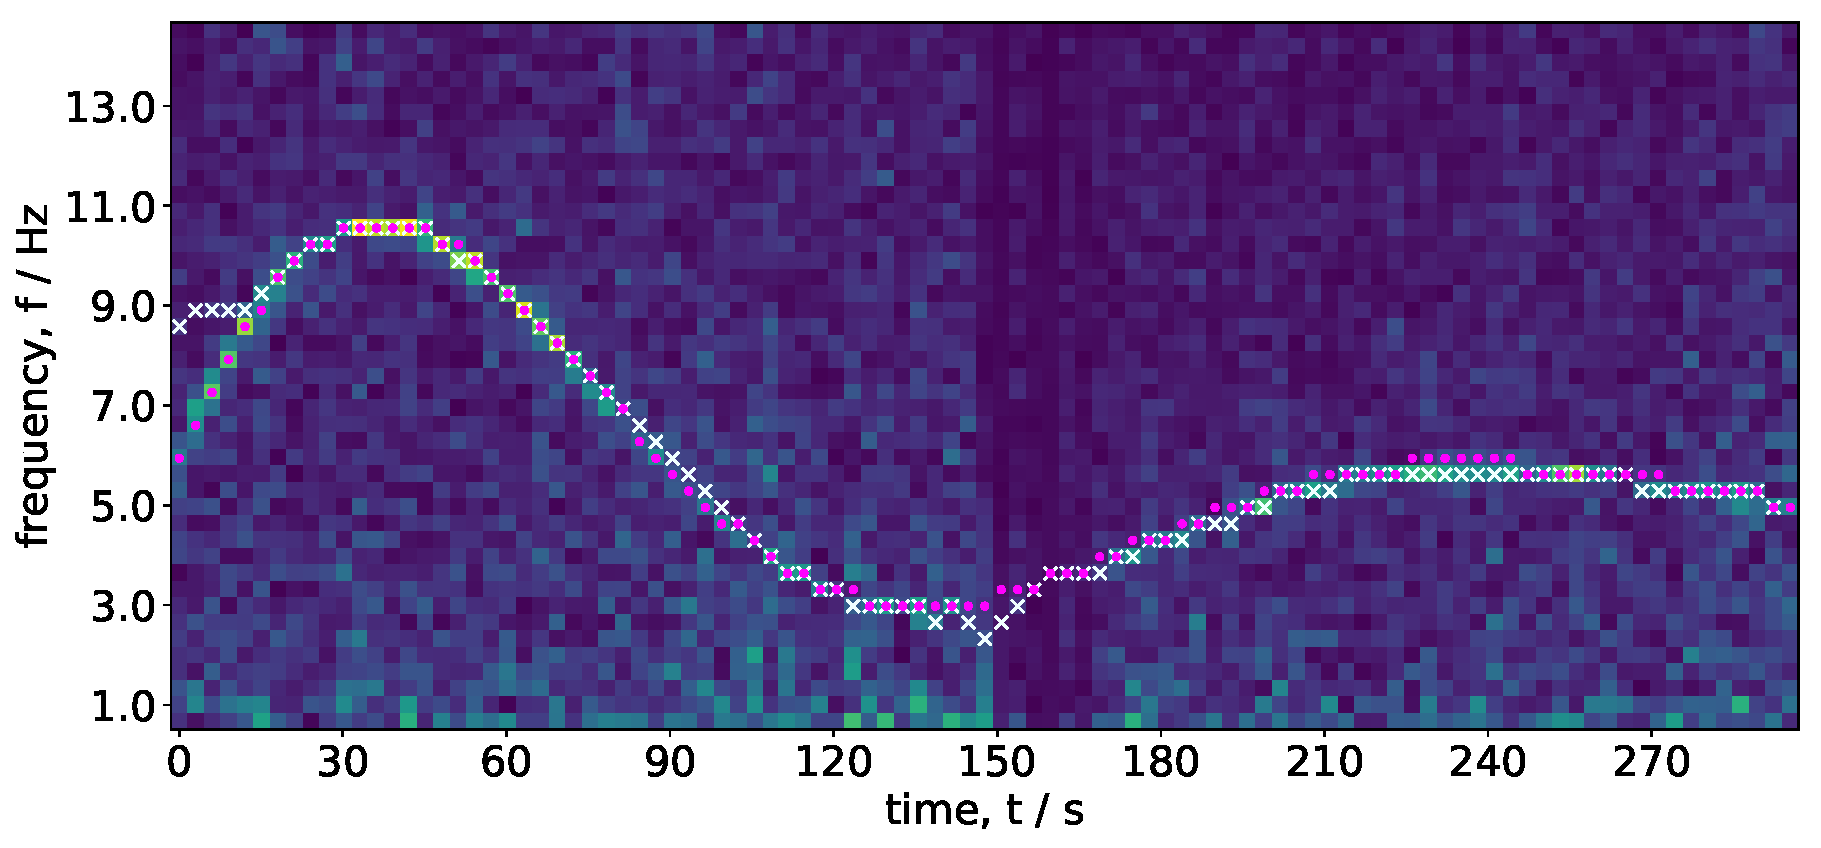
\includegraphics[width=\textwidth]{figures/expt_overlay_2_viterbi_test_webcam.pdf}
	\caption{Spectrogram of observed signal overlaid with white crosses for the Viterbi path and pink dots for the injected signal, notice the high correlation between them indicating that the signal is able to be recovered; also note the deviation at the start when the signal moves too quickly and just before the background anomaly at 150s}
	\label{fig:viterbi_overlay}
\end{figure}

\section{Complex audio}
\label{sec:optical_microphone}
% Optical microphone
% aim of optical microphone: play back injected sounds

The natural succession to simple tones is to study complex audio signals, such as music and speech.
The Viterbi algorithm and tracking more broadly is not applicable to these signals. Compare a single tone that slowly, continuously changes frequency to music and speech which consist of a broad spectrum that is constantly changing.
Instead, the interest here is in being able to record and play-back these complex audio signals, rather than track them. Using the interferometer to do so makes it, in ensemble with the measuring device, an ‘optical microphone’, using light to capture sound.


Advanced signal processing is required to extract gravitational wave signals from very noisy observational data. Recovering audio from an optical microphone requires related signal processing. Although far simpler, it serves as another useful demonstration.

\subsection{The photodiode method}
\label{sec:photodiode}
% advanced method: explain how we capture data

For an optical microphone to be sensitive to speech and music it needs a frequency response far higher than the 30Hz of a standard webcam. Both speech and music need at least kHz range, with speech intelligibility requiring up to 3kHz and music preferably up to and beyond 8kHz. This can be addressed by using a high-speed webcam, or more simply, by using a photodiode as the measuring device.


A photodiode is an electrical component that acts as a regular diode (blocking any current flow in the reverse direction) when no light is incident on it, but becomes more and more conductive in the reverse direction as the intensity of incident light increases. 
Fundamentally, a current is created in the photodiode by the photo-electric effect. Placing a photodiode in reverse-bias over an op-amp creates a photo-detector that will produce a voltage dependent approximately linearly to the incident intensity. \jam{How sound is this approximation?} This experiment had the photodiode in the interference pattern at roughly the same spot as the webcam was monitoring previously, just off-centre.


The voltage signal from the photo-detector is captured by a 10-bit analog-to-digital converter (ADC) connected to the special purpose input (SPI) pins of a Raspberry Pi, in the standard configuration. This digitally samples the signal at roughly 16kHz. As such, any frequency component of the analog signal above the Nyquist frequency of 8kHz would be aliased down into the detected range.
To prevent this, an anti-aliasing Sallen-Key filter tuned to 16kHz is included before the ADC. This component attenuates any frequencies above 8kHz, before they get digitally sampled.
It’s not immediately clear what’s limiting the sample rate to 16kHz, but it is likely non-optimal reading of the ADC by the Pi script.
% The ADC used (MCP3008) is quoted at 200kHz (or ksps, kilo samples per second).


The entire circuit diagram is detailed and shown in Appendix~\ref{app:circuit_diagram}. The updated schematic is shown in Figure~\ref{fig:ifo_schematic_podo} and a picture taken of the experiment, showing the interferometer, the circuit, and the Pi, is shown in Figure~\ref{fig:setup_pic2}.

\begin{figure}
	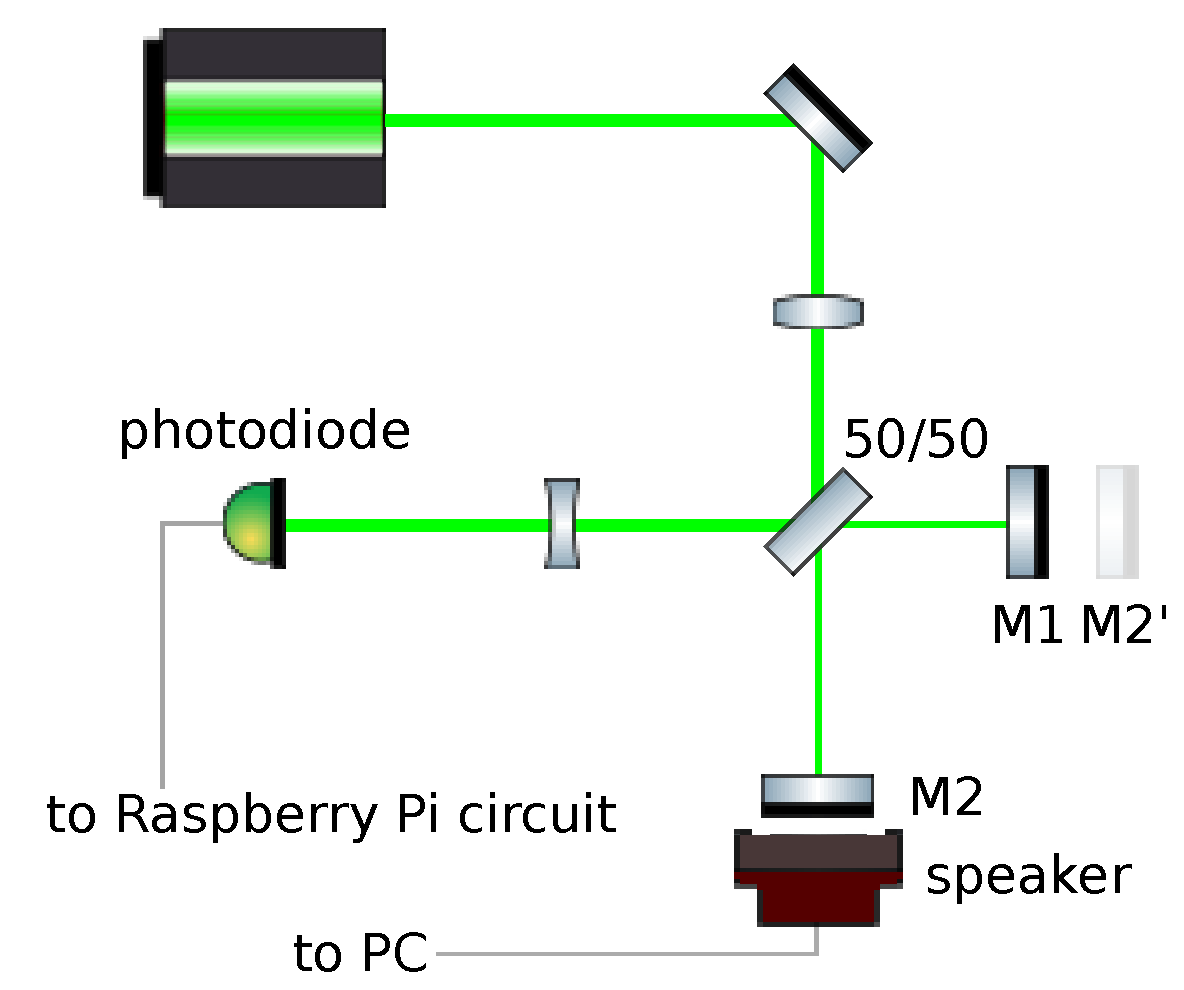
\includegraphics[width=0.8\textwidth]{figures/ifo_schematic_photodiode.pdf}
	\caption{Michelson interferometer schematic, a part of the interference pattern is recorded by a photodiode}
	\label{fig:ifo_schematic_podo}
\end{figure}

\begin{figure}
	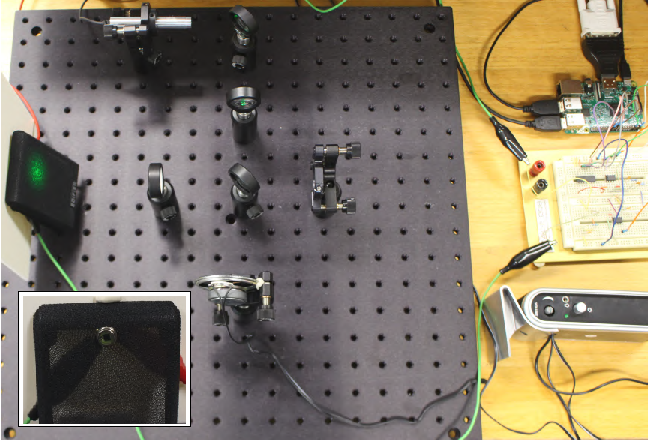
\includegraphics[width=\textwidth]{figures/setup_pic2.pdf}
	\caption{Picture taken of the optical microphone set-up, showing the Michelson interferometer, the photodiode (in an insert), the circuit, and the Raspberry Pi.}
	\label{fig:setup_pic2}
\end{figure}

\subsection{Initial results}
% breakdown of all the filters used along the way

The optical microphone was tested on recordings of one human talking and on music ranging from simple melodies to full tracks. Each recording was around one minute long with processing done on ten second segments. For each observation, the audio was played through the speaker with minimal activity around interferometer as the Pi script recorded the signal. The saved time series was then directly converted to a .wav file and played as an audio recording, using the \textbf{scipy.io.wavfile.write}\cite{scipy} implementation in Python\cite{python}.


These initial recordings were extremely noisy and painful to listen to, with a loud bass sound throughout. Spectra of all of these recordings showed a dominant mains hum at 50Hz with strong power up to and beyond the 8th harmonic thereof. This power is also present with the speaker off, as is shown in Figure~\ref{fig:psd_noise}, and also weakly when monitoring with the photodiode in complete darkness.

\begin{figure}%[H]
	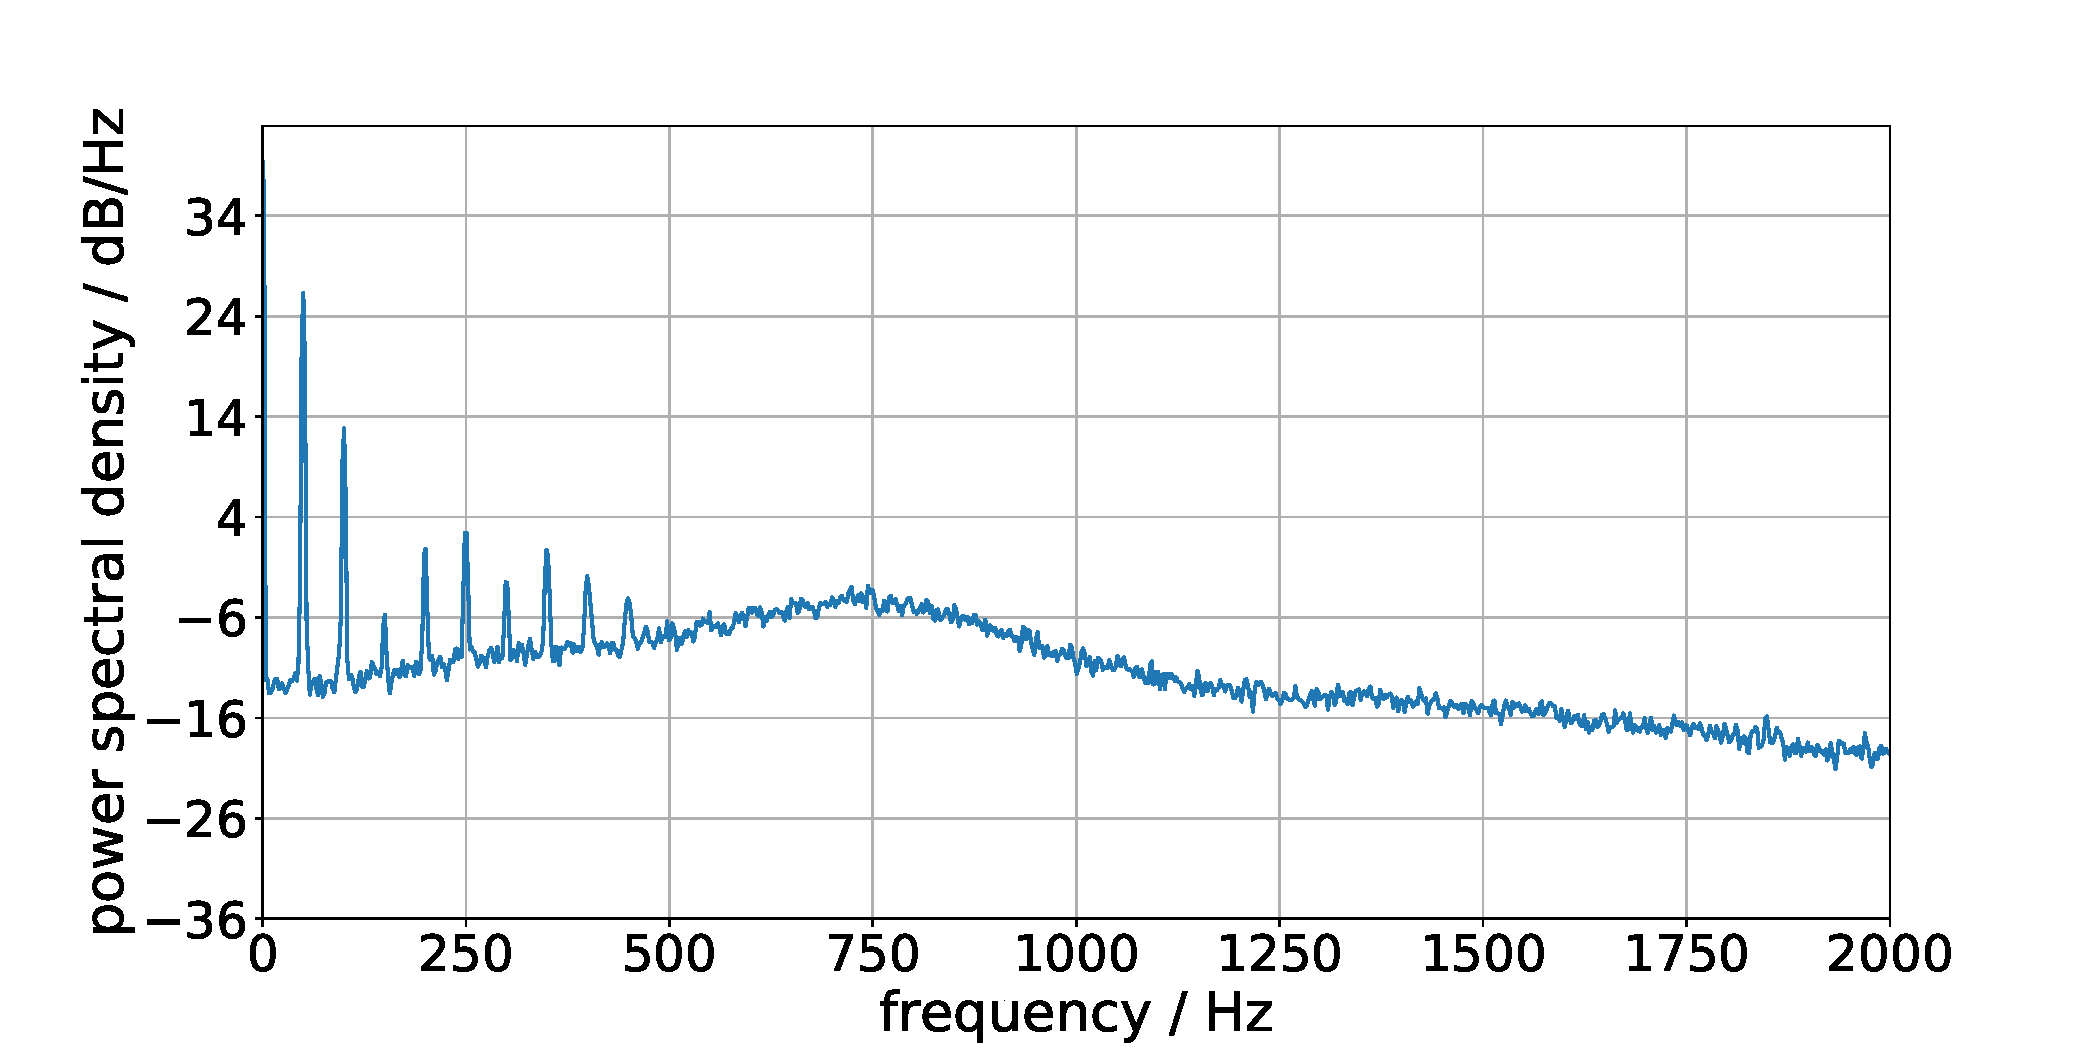
\includegraphics[width=\textwidth]{figures/podo_noise_psd_zoom-cropped.pdf}
	\caption{Power spectral density (PSD) of the optical microphone system with no injected audio (i.e.\ with the speaker off), show high power in the 50Hz mains hum and its harmonics (most likely from the photodiode circuit and the ambient lighting), otherwise is a fairly white spectrum except for the broad, shallow maximum at 750Hz}
	\label{fig:psd_noise}
\end{figure}

\subsection{Filters applied}

Early attempts to remove the mains hum included zeroing the channel of each 50Hz harmonic, this is effectively using a rectangular comb filter. Applying a filter (multiplying by a function) in frequency space is equivalent to convolving the signal with the inverse Fourier transform of that filter. While this did remove the mains harmonics, it also destroyed the rest of the signal.


Attempting to low-pass the signal did better (to the ear) but was also problematic as the harmonics are all over the 100Hz-1kHz region, which also carries a lot of the speech and music information. Low-passing the logarithm of the signal and then converting back did better still but doesn’t significantly remove the mains noise.


Of these simple filters, the best performing was a band-pass Butterworth filter with frequency response shown in Figure~\ref{fig:butterworth}. This filter is `maximally flat' within the band region, here 150Hz to 3kHz, and trails off outside of the band with slope dependent on the order of the filter, here of order 5. This still suffered from the presence of the higher mains harmonics. However, behind the remaining noise one could hear something distinctly speech-like or musical, just with very low intelligibility, you couldn’t understand the speech but could recognise that someone was talking.


Note that we also replicated the Viterbi algorithm results from before with the photodiode, but only with the mains hum removed and high-passing above 100Hz, else the algorithm never selected the signal. Except for being over audible frequencies, there isn’t much difference in the tracking once these filters are applied.

\begin{figure}%[H]
	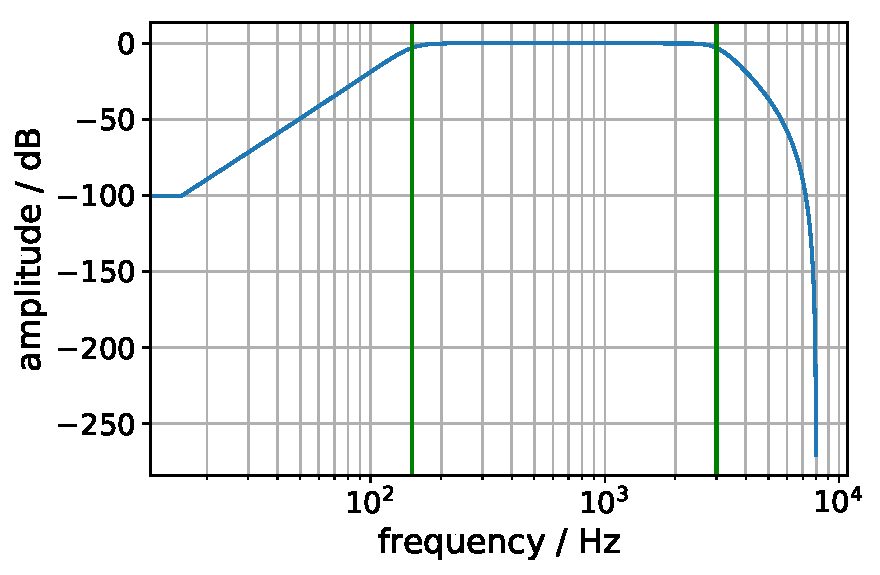
\includegraphics[width=0.8\textwidth]{figures/butterworth_150_3000-cropped.pdf}
	\caption{Butterworth bandpass filter frequency response, green vertical lines show the band limits of 150Hz and 3kHz. Note the very flat response within the band, any amplitude beyond -3dB is significant attenuation.}
	\label{fig:butterworth}
\end{figure}

\subsection{logMMSE estimator}
% logMMSE

\jam{Explain MMSE as in the second talk, be honest in some way}

Speech enhancement for a noisy channel is a classic problem in signal processing. Hu~\&~Loizou~(2006)~\cite{SubjectiveComparison} compare various methods and find the best performing statistical technique to be the logMMSE (alt.\ MMSE-LSA) estimator which minimises the mean square error (MSE) of the log-spectral amplitude. This means that it takes the logarithm of the spectrum of the original signal and finds the fit (or estimate) that has the minimal MSE to that log-spectra.
% Use of the logarithm is a common technique in speech processing as it, somewhat surprisingly, does not significantly change the intelligibility to the human ear.


Applying an existing implementation of logMMSE\cite{logmmse} to the optical microphone recordings produces dramatically cleaner results. The time series and spectrum from before and after the logMMSE filter is applied are shown in Figures~\ref{fig:logMMSE_timeseries}~\&~\ref{fig:logMMSE_spectrum}. All of the mains harmonics are significantly attenuated. And further high-passing removes the low frequency curve beneath 100Hz.


There is varied success with passing music passed through the filters. Loud, rhythmic chords and drums are received well and remain recognisable, while thinner, airy flute and violin melodies struggle to be heard in the results. It is likely that the lower sounds have higher amplitude speaker oscillations and so pass through the optical microphone better.


However, speech intelligibility remains very low with the voice sounding mumbled and indistinct. Enhancement so far has removed most of the background sound, as evidenced by the near silence between words, but has not clarified the speech. There is a question here as to where the diction in the speech is lost, at the speaker-mirror coupling, at the photodiode reading, or if it is still there, just obscured in the noisy signal.

% The fringe counting problem of the detector, wherein multiple fringes passing over the array in a single speaker deflection artificially raises the frequency, was noticeable in the speech recordings when compared to the source audio. However, upon comparing injected pure tones, the increase appears to be minimal and inconsistent, at around 5Hz maximum difference. An simple explanation is that the speaker deflections are small compared to manual pressing on the optical table.
% Visually it is impossible to confirm this for high frequencies, but it remains possible.

\begin{figure}%[H]
	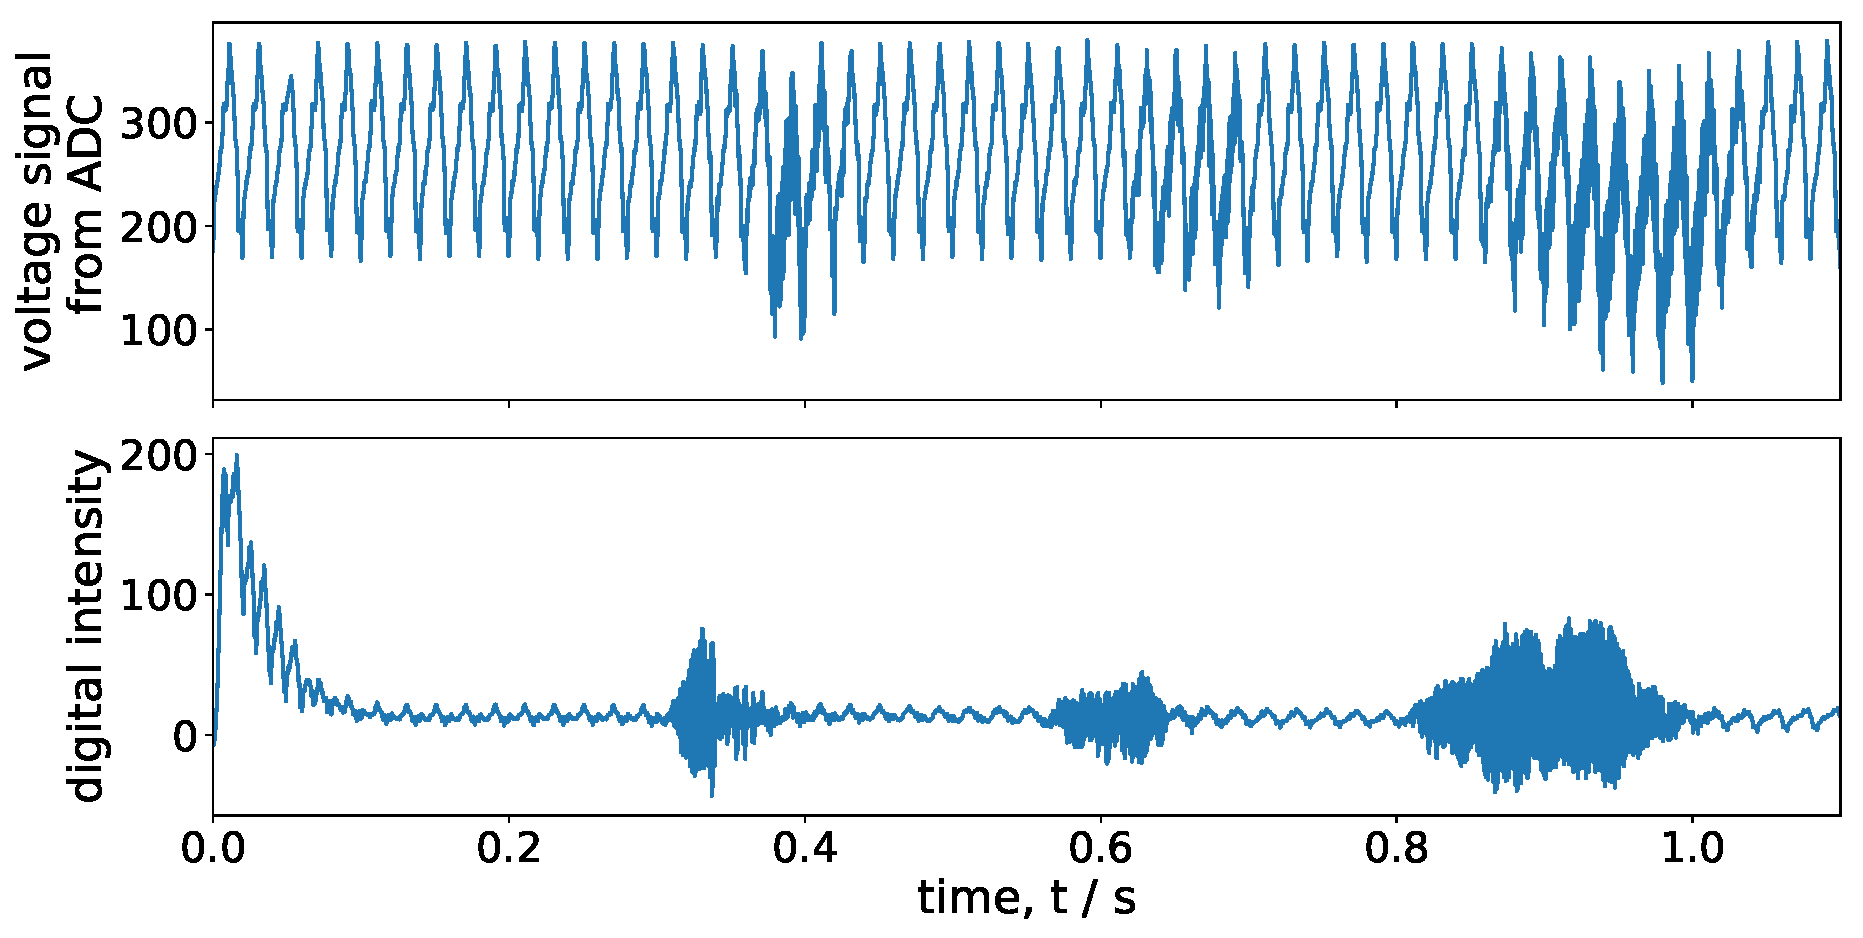
\includegraphics[width=\textwidth]{figures/filter_timeseries_aa_melatos-cropped.pdf}
	\caption{Optical microphone recording of adult male voice (saying ``A cathode ...'') shown before (top) and after (bottom) logMMSE filter is applied, only one second of the one minute recording is shown. The bump at the start of the time series is the result of filtering a finite signal, and is expected.}
	\label{fig:logMMSE_timeseries}
\end{figure}

\begin{figure}%[H]
	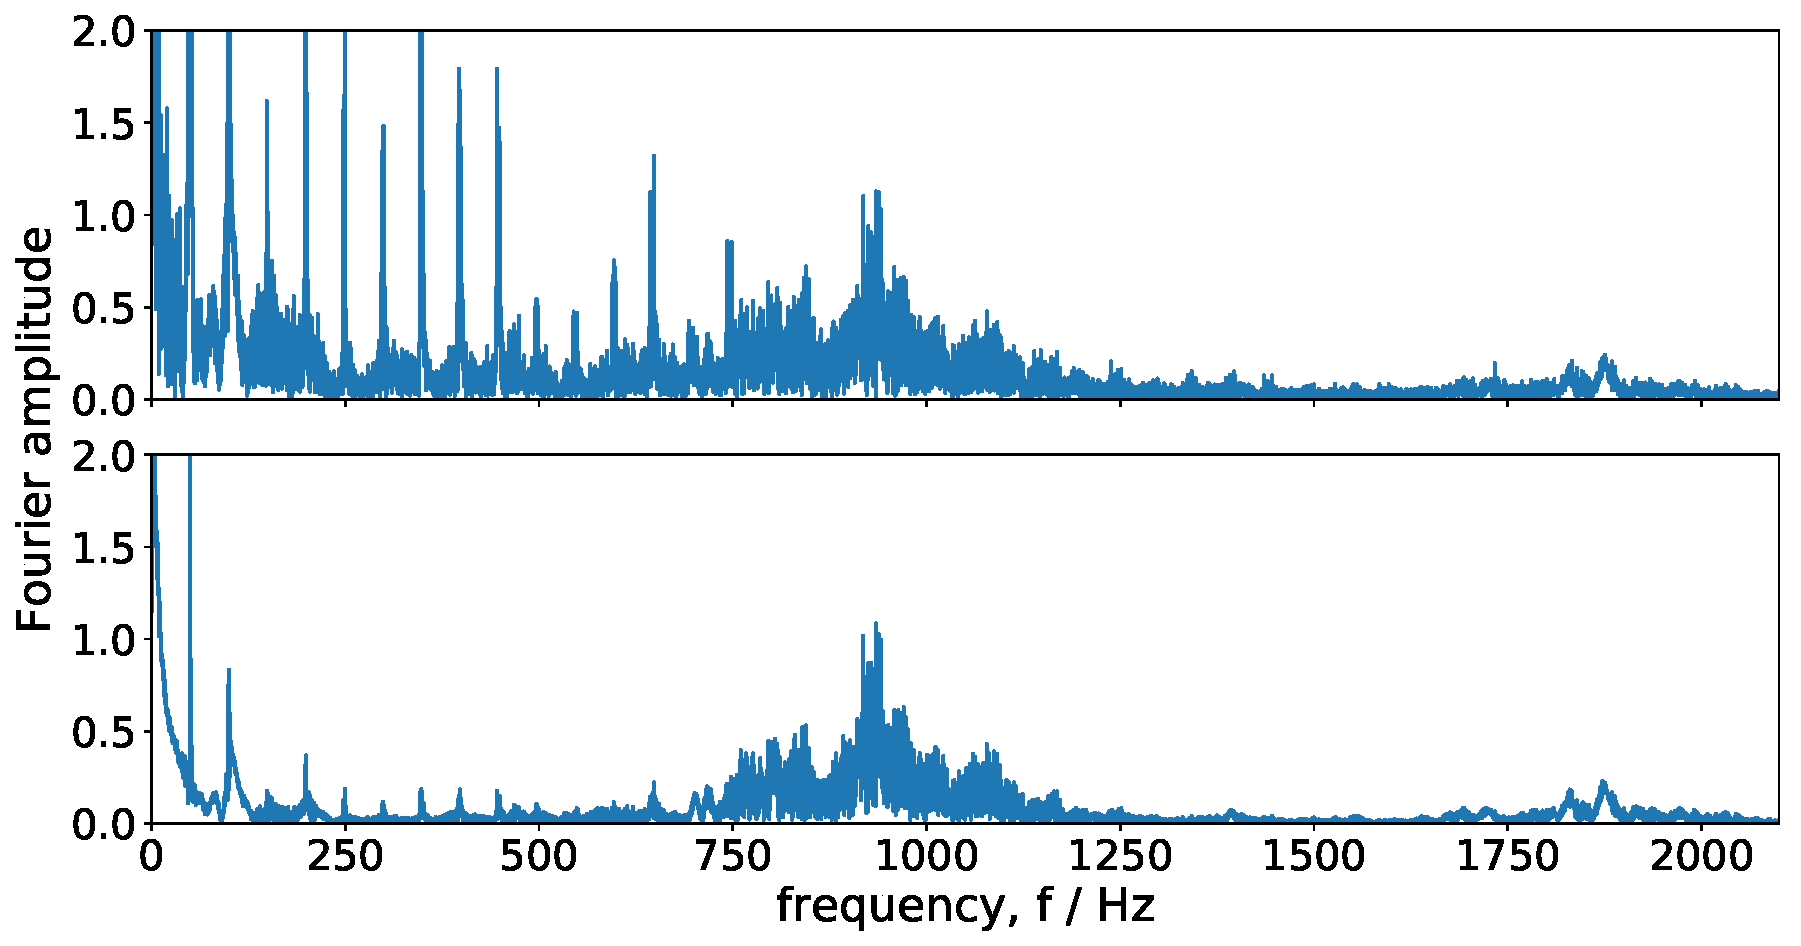
\includegraphics[width=\textwidth]{figures/filter_spectrum_aa_melatos-cropped.pdf}
	\caption{Spectrum of optical microphone recording of adult male voice shown before (top) and after (bottom) logMMSE filter is applied, showing only up to 2kHz and a detail of the spectrum (limited to show only up to amplitude 2, while before filtering the 50Hz line has an amplitude of 40)}
	\label{fig:logMMSE_spectrum}
\end{figure}


\section{Future work}
\label{sec:future_work}

\jam{BATTERY POWER}
% any other wild speculation?

\subsection{Transfer function}

The intensity, $I$, of the interference pattern at a particular angle is given by Equation~\ref{eq:intensity_result} below. Where A is the amplitude of the electric field of the beam, d is the separation (or the difference in the arm lengths), $\theta$ is the angle from the centre-line to the point on the screen, and $\lambda$ is the wavelength, 532nm, of the laser (see Appendix~\ref{app:intensity_derivation} for the derivation to get to this equation).
\begin{equation}
\label{eq:intensity_result}
I = 2 A^2 (1+\cos{\phi}), \; \phi = \frac{4 \pi d \cos{\theta}}{\lambda}
\end{equation}

This Equation~\ref{eq:intensity_result} means that the intensity changes non-linearly with a small change in separation, as in Equation~\ref{eq:intensity_change} (see Appendix~\ref{app:intensity_derivation} again for the derivation). This makes the problem of extracting the original signal more difficult.

\begin{equation}
\label{eq:intensity_change}
	\frac{\delta I}{\delta d} = \frac{- 8 \pi A^2 \cos{\theta}}{\lambda} \sin{(\frac{4 \pi \cos{\theta}}{\lambda} d)}
\end{equation}

A full model of the transfer function would detail the system starting from the voltage sent to the speaker and ending with the value recorded by the Pi, including any non-linearities in the speaker audio production, the speaker-mirror coupling, the separation-intensity relation, and the photodiode reading. Although we have the separation-intensity relation as non-linear for small motions (see above), the other components of this full model are yet to be determined. Figure~\ref{fig:pipeline_highlighted} shows this full pipeline, with the currently determined section highlighted.


Theoretically, if we had the correct model, then signal recovery would only be limited by the SNR. We could also use long recordings of white noise to estimate a matched filter for the system.


For further speech enhancement, the optimal filter would involve a hidden-Markov-model trained to English phonemes. Alternatively, machine learning solutions also exist through-out the field.


\begin{figure}%[H]
	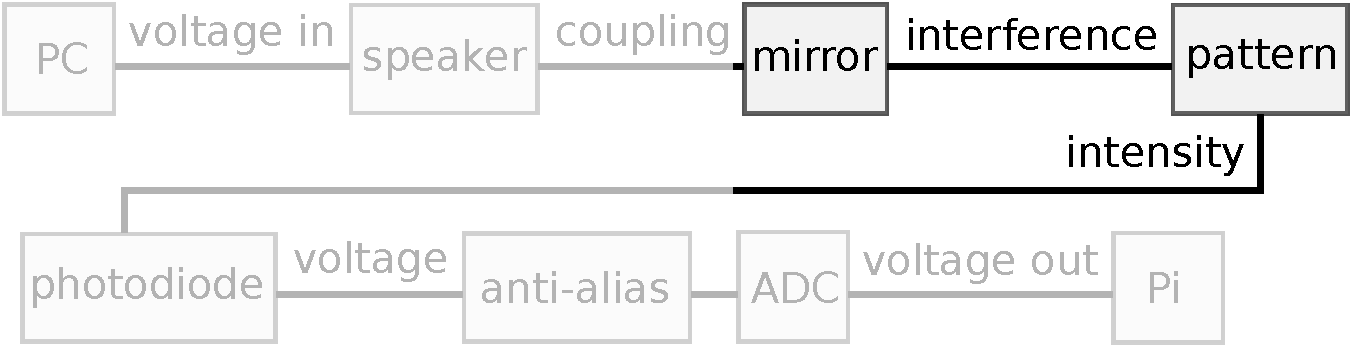
\includegraphics[width=\textwidth]{figures/pipeline_highlighted.pdf}
	\caption{???}
	\label{fig:pipeline_highlighted}
\end{figure}


\section{Conclusions}
\label{sec:conclusions}

Using a Michelson interferometer, we able to successfully demonstrate the Viterbi algorithm recovering an injected signal. Just as is done is continuous gravitational wave searches. We are also able to play-back chordal or rhythmic music from an optical microphone (using the same interferometer), while recordings of simple speech are audible but unintelligible.

\newpage
\appendix

\section{Open-source code}
\label{app:code}
This project is implemented in python3\cite{python} inside of jupyter notebooks\cite{jupyter}\cite{ipython} and uses the packages of numpy\cite{numpy}, scipy\cite{scipy}, matplotlib\cite{matplotlib}, tqdm\cite{tqdm}, and logmmse\cite{logmmse}.

The current build can be found at:
\url{https://github.com/daccordeon/gravexplain}
% \begin{verbatim}
% README
% \end{verbatim}

\section{Additional guide to reproducing results}
\label{app:reproducing_results}
% as for a 3rd year undergraduate

Besides the directions given in the rest of this article, there are some observations and technical details useful to someone wanting to reproduce the results shown herein. For the analysis and signal processing performed the best reference is Appendix~\ref{app:code} for the open-source code.

For the experiment, since a Michelson interferometer is such a standard configuration, we’ll not detail it further here, see any optics manual for more information. To obtain an independent speaker cone we recommend carefully dismantling a budget commercial speaker system to get at the speaker within. To attach the speaker to one of the mirrors, we wedged it into part of the mirror mount and used commercial adhesive putty to keep it in place. If the other speaker in the pair remains, keep it as far away from the experiment and as damped as possible else it may act as a second, interfering source.
% we used a Class 2 LDS5 ThorLabs laser at 532nm

For the photodiode circuit, we used a Raspberry Pi and an MCP3008 ADC to monitor the analog signal. This could also be done with the analog pins on an Arduino. Be careful of the gain through the LM358 op-amps in the circuit though, else the ADC in either case could threshold the signal. Also be ready to change the values in the Sallen-Key filter to match your own sampling rate. The photodiode was an OSRAM BPW21, we mounted it through a discarded piece of speaker mesh (similar to black cloth over a frame) and placed another piece over the face to not over expose and threshold the signal. For the rest of the circuit, we used standard components assembled as in \ref{app:circuit_diagram}.

\jam{Add this in, lots of advice and detail!}


\section{The Viterbi Algorithm}
\label{app:viterbi}

To find the Viterbi path through a spectrogram (spectra over time), given an M x N grid of M frequency rows and N time columns and a rate limit for the change of frequency over time that we convert into the number of allowed rows we can move while stepping from each column to the next (this limit was $\pm 1$ row/column in our case). The path must start from the first column and end at the last, taking a single step in each column along the way. Each element in the grid is the norm of the Fourier component of a frequency at a time. These are normalised between $(0, 1)$ to use as multiplicative weights, i.e.\ the total weight of a path is the product of all weights along that path. In fact, we take the logarithm and so the sum of all weights to avoid underflow. The best path has the highest weight.


With the grid prepared, the Viterbi algorithm starts in the second column. In each iteration, the algorithm looks for the best path to each cell from the cells in the previous column, taking the greatest cumulative weight of those available, ‘nearby’ cells (the value of which was discovered in the previous iteration).
For each cell in the current column, the algorithm notes this weight plus the cell’s own weight, along with the row index of which cell in the previous column it came from.
Continuing like this until it reaches the end of the grid, the algorithm then looks for the greatest weight in the last column and retraces the indices of the steps it took until it reaches the start of the grid. That best path is the Viterbi path.


\section{Common wandering frequency mistake}
\label{app:phase_gotcha}

We want to generate a sine wave that changes frequency over time so that the frequency at some time is given by a function $f(t)$. The common mistake is to just appeal to the standard form $\sin{(2 \pi f t)}$, where f would be a constant frequency, and write down $\sin{(2 \pi f(t) t)}$. However, accumulation of phase means that this produces a curve that looks very different to that desired. Instead, one should see that the standard form in fact says that for some $\sin{(F(t))}$ it is true that $\frac{dF}{dt}(t) = 2 \pi f(t)$, where $f(t)$ gives the frequency of $\sin{(F(t))}$ at time $t$. Therefore, the correct form for a wandering tone is $\sin{(\int{2 \pi f(t) dt})}$.


\section{Circuit design}
\label{app:circuit_diagram}
% schematic of breadboard and connections to pi
% https://www.circuit-diagram.org/editor/
% https://crcit.net/c/e397dcc2166943d69155f9dac1e27bce

Figure~\ref{fig:circuit_diagram} shows the photodiode circuit diagram, it is also available at \url{https://crcit.net/c/e397dcc2166943d69155f9dac1e27bce}

\begin{figure}%[H]
	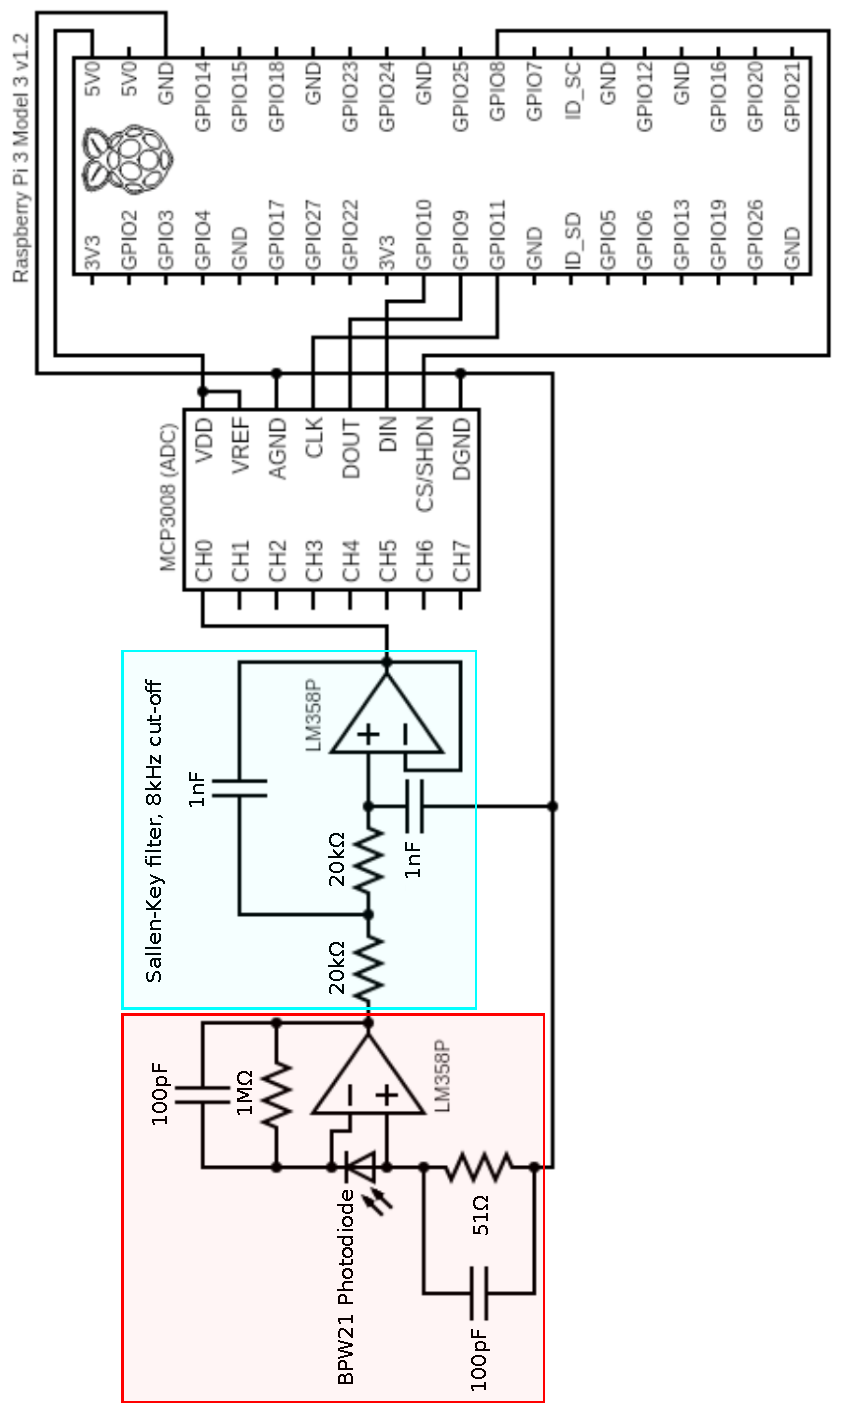
\includegraphics[width=\textwidth]{figures/circuit_diagram_2.pdf}
	\caption{Circuit diagram for photodiode reading. Photodiode in reverse-bias over an op-amp, analog signal then passed through Sallen-Key anti-aliasing filter tuned to 16kHz, then into an analog-to-digital converter (ADC), that’s finally read by the special purpose input (SPI) pins of a Raspberry Pi}
	\label{fig:circuit_diagram}
\end{figure}


\section{Intensity relation derivation}
\label{app:intensity_derivation}

We want the change in intensity, $\delta I$, at a point in the Michelson interference pattern, given a small change, $\delta d$, in the perpendicular path difference of the mirrors (or in the separation of one and virtual image of the other). The point is at angle $\theta$ on the screen above the central ray, noting circular symmetry. At this point, two rays meet, one from each mirror, with the total electric field (\jam{parallel to the screen?}) being $E_1(t) + E_2(t)$. Given an initial separation of $d$, the path difference between the mirrors is $2 d \cos{\theta}$ as the longer ray must travel to and from the further mirror, and both move up at the angle $\theta$ to meet at the screen.

\begin{align}
\label{eq:intensity_derivation}
    E_1(t) &= A e^{i (k L - \omega t)} \\
    E_2(t) &= A e^{i (k (L + 2 d \cos{\theta}) - \omega t)} \\
    I(t) &= \lvert A e^{i (k L - \omega t)} + A e^{i (k (L + 2 d \cos{\theta}) - \omega t)} \rvert^2
\end{align}

Collapse the phase difference to $\phi$ and expand the norm squared by expanding the complex exponentials. From there is it trigonometric manipulation to reach the result of intensity in terms of separation.

\begin{align}    
    I(t) &= A^2 \lvert e^{i (k L - \omega t)} + e^{i (k L + \phi - \omega t)} \rvert^2,\, \phi = 2 k d \cos{\theta} \\
    I(t) &= A^2 ((\cos{(k L - \omega t)} + \cos{(k L + \phi - \omega t)})^2 + (\sin{(k L - \omega t)} + \sin{(k L + \phi - \omega t)})^2) \\
    I(t) &= A^2 (1 + 2 \cos{(k L - \omega t)} \cos{(k L + \phi - \omega t)} + 1 + 2 \sin{(k L - \omega t)} \sin{(k L + \phi - \omega t)}) \\
    I(d) &= 2 A^2 (1 + \cos{\phi}),\, \phi = \frac{4 \pi d \cos{\theta}}{\lambda}
\end{align}

Then take derivatives and find that the intensity change is non-linear.

\begin{align}    
    \frac{\delta I}{\delta d} &= \frac{\delta I}{\delta \phi}\; \frac{\delta \phi}{\delta d}\\
    \frac{\delta I}{\delta\phi} &= - 2 A^2 \sin{\phi}\\
    \frac{\delta\phi}{\delta d} &= \frac{4 \pi \cos{\theta}}{\lambda}\\
    \therefore \frac{\delta I}{\delta d} &= \frac{- 8 \pi A^2 \cos{\theta}}{\lambda} \sin{(\frac{4 \pi \cos{\theta}}{\lambda} d)}
\end{align}


\begin{acknowledgments}
The authors are grateful to Jude Prezens, Alex Tolotchkoc, and Blake Molyneux for their technical advice and generous assistance throughout the project.
	
The authors are also grateful to Deeksha Beniwal, Sebastian Ng, and Craig Ingram for their advice and work in designing the interferometer. 

This research is supported by the Australian Research Council Centre of Excellence for Gravitational Wave Discovery (OzGrav) (project number CE170100004) and the Institute of Physics International Member Grant.

Travel during the project was supported by the Australian National University PhB Science  program.

\end{acknowledgments}


\bibliographystyle{myunsrt}
\bibliography{ifoDemoBib}

\end{document}
